\documentclass[11pt, a4paper]{report}

%====================== PACKAGES ======================

\usepackage[french]{babel}
\frenchbsetup{StandardLists=true}
\usepackage{enumitem}
\usepackage{pifont}
\usepackage[utf8x]{inputenc}
%pour gérer les positionnement d'images
\usepackage{float}
\usepackage{amsmath}
\DeclareMathOperator{\dt}{dt}
\usepackage{graphicx}
\usepackage{tabularx}
\usepackage[colorinlistoftodos]{todonotes}
\usepackage{url}
%pour les informations sur un document compilé en PDF et les liens externes / internes
\usepackage[pdfborder=0]{hyperref}
\hypersetup{
	colorlinks = true
	}
%pour la mise en page des tableaux
\usepackage{array}
\usepackage{tabularx}
\usepackage{multirow}
\usepackage{multicol}
%pour utiliser \floatbarrier
%\usepackage{placeins}
%\usepackage{floatrow}
%espacement entre les lignes
\usepackage{setspace}
%modifier la mise en page de l'abstract
\usepackage{abstract}
%police et mise en page (marges) du document
\usepackage[T1]{fontenc}
\usepackage[top=2cm, bottom=2cm, left=2cm, right=2cm]{geometry}
%Pour les galerie d'images
\usepackage{subfig}

\usepackage{pdfpages}

%====================== INFORMATION ET REGLES ======================

%rajouter les numérotation pour les \paragraphe et \subparagraphe
\setcounter{secnumdepth}{4}
\setcounter{tocdepth}{4}

\hypersetup{							% Information sur le document
pdfauthor = {Stephan Runigo},			% Auteurs
pdftitle = {Documentation simulateur de foule},			% Titre du document
pdfsubject = {Documentation du simulateur de foule},		% Sujet
pdfkeywords = {simulateur de foule, C, sdl2},	% Mots-clefs
pdfstartview={FitH}}	% ajuste la page à la largeur de l'écran
%pdfcreator = {MikTeX},% Logiciel qui a crée le document
%pdfproducer = {} % Société avec produit le logiciel
%======================== DEBUT DU DOCUMENT ========================
%
\begin{document}
%
%régler l'espacement entre les lignes
\newcommand{\HRule}{\rule{\linewidth}{0.5mm}}
%
%page de garde
%\begin{titlepage}
\begin{center}

% Upper part of the page. The '~' is needed because only works if a paragraph has started.
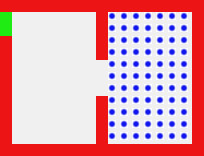
\includegraphics[width=.35\textwidth]{./titre/SimFoule0104}
%\caption{SiCF}
\label{fig:image1}
~\\[1cm]

\begin{figure}[htbp]
\begin{minipage}[c]{.45\linewidth}
\begin{center}
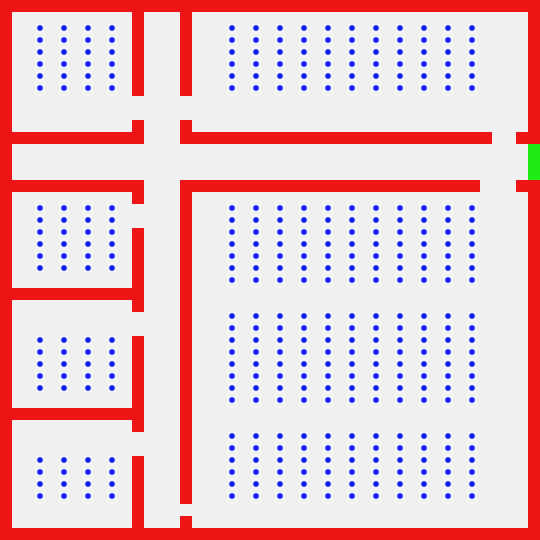
\includegraphics[scale=0.35]{./titre/SimFoule0103}
%\caption{SiCF}
%\label{fig:image1}
\end{center}
\end{minipage}
\hfill
\begin{minipage}[c]{.45\linewidth}
\begin{center}
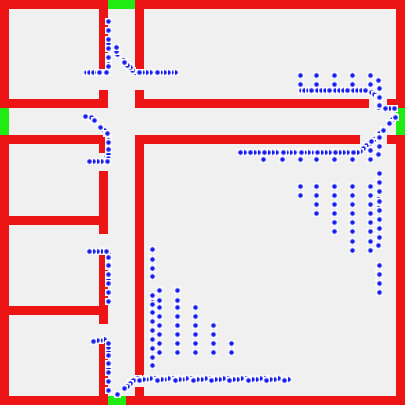
\includegraphics[scale=0.45]{./titre/SimFoule0105}
%\caption{diagramme des tâches.}
%\label{SiCP}
\end{center}
\end{minipage}
\end{figure}
%\textsc{\LARGE Complément nutritionnel}\\[1.5cm]
~\\[1cm]

\textsc{\Large }\\[0.5cm]

% Title
\HRule \\[0.4cm]

{\huge \bfseries  SimFoule 2.2\\[0.2cm] 
Documentation et théorie\\[0.4cm] }

\HRule \\[1.5cm]

% Author and supervisor
\begin{minipage}{0.4\textwidth}
\begin{flushleft} \large
%\emph{Auteur:}\\
%Stephan \textsc{Runigo}
\end{flushleft}
\end{minipage}
\begin{minipage}{0.4\textwidth}
\begin{flushright} \large
\emph{Auteur:}\\
Stephan \textsc{Runigo}
\end{flushright}
\end{minipage}

\vfill

% Bottom of the page
{\large \today}

\end{center}
\end{titlepage}

%
%page blanche
\begin{center}
\Large
Résumé
\normalsize
\end{center}
\vspace{3cm}
\begin{itemize}[leftmargin=1cm, label=\ding{32}, itemsep=21pt]
\item {\bf Objet : }Ce document (en cours de construction), accompagne le programme SimFoule (lui même en cours de développement).
\item {\bf Contenu : }Il contient un manuel d'installation et d'utilisation ainsi que quelques développements théoriques liés à ce programme de simulation.
\item {\bf Public concerné : }Ce document s'adresse aux enseignants et aux étudiants du supérieur des sections sciences physiques et informatique. Il s'adresse également à tout les passionnés d'informatique et de la langue de Molière.
\end{itemize}

\vspace{3cm}

SimFoule est un simulateur numériques de foule offrant une représentation graphique et une interaction dynamique avec les paramètres physiques. Destinés à un usage pédagogique, il permet de visualiser le comportement d'une foule lors d'une évacation. Cette documentation accompagne ce programme.

\begin{itemize}[leftmargin=1cm, label=\ding{32}, itemsep=11pt]
\item Le premier chapitre présente le simulateur, fourni une procédure d'installation et précise les commandes permettant l'interaction avec le programme.
\item Le chapitre suivant fourni un certain nombre de développements théoriques liés à la modélisation physique des foules.
\item Enfin, le dernier chapitre rassemble les informations liées à la structure du programme.
\end{itemize}

%\newpage
%~
%ne pas numéroter cette page
%\thispagestyle{empty}
\newpage

\tableofcontents
\thispagestyle{empty}
\setcounter{page}{0}
%ne pas numéroter le sommaire
%
%\newpage
%
%espacement entre les lignes d'un tableau
\renewcommand{\arraystretch}{1.5}
%
%====================== INCLUSION DES PARTIES ======================
%
~
\thispagestyle{empty}
%recommencer la numérotation des pages à "1"
\setcounter{page}{0}
\newpage
%
%
\chapter{Installation et utilisation}
%

%%%%%%%%%%%%%%%%%%%%%%%%%%%%%%%%%%
%
%%%%%%%%%%%%%%%%%%%%%%%%%%%%%%%%%%

\section{Présentation du simulateur}
%
Le simulateur SimFoule est un programme informatique écrit en C et qui utilise la librairie SDL2. Il donne une représentation graphique d'une foule se déplaçant dans un batiment. Une évacuation du batiment peut être déclenchée.
%
%
\section{Installation du simulateur}
Cette section traite de l'installation du simulateur SimFoule sur un système d'exploitation de type debian. Le téléchargement se fait avec un navigateur internet, la compilation et l'exécution se font dans un terminal. L'installation des outils de compilation nécessite les privilèges du super-utilisateur.
\begin{itemize}[leftmargin=1cm, label=\ding{32}, itemsep=0pt]%\end{itemize}
\item {\bf Installation des outils de compilation}
	\begin{itemize}[leftmargin=1cm, label=\ding{32}, itemsep=0pt]
	\item \texttt{sudo apt-get install gcc make libsdl2-dev}
	\end{itemize}
\item {\bf Téléchargement des sources}
	\begin{itemize}[leftmargin=1cm, label=\ding{32}, itemsep=0pt]
	\item Télécharger le fichier \texttt{.zip} sur github
		\begin{itemize}[leftmargin=1cm, label=\ding{32}, itemsep=0pt]
		\item \texttt{https://github.com/runigo/SimFoule/archive/master.zip}
		\end{itemize}
	\item Décompresser le fichier \texttt{.zip}
		\begin{itemize}[leftmargin=1cm, label=\ding{32}, itemsep=0pt]
		\item \texttt{unzip SimFoule-master.zip}
		\end{itemize}
	\end{itemize}
\item {\bf Compilation}
	\begin{itemize}[leftmargin=1cm, label=\ding{32}, itemsep=0pt]
	\item La commande \texttt{make} dans le répertoire des sources produit un fichier exécutable :
		\begin{itemize}[leftmargin=1cm, label=\ding{32}, itemsep=0pt]
		\item \texttt{SimFoule}
		\end{itemize}
	\end{itemize}

\item {\bf Exécution}
	\begin{itemize}[leftmargin=1cm, label=\ding{32}, itemsep=0pt]
	\item En ligne de commande, avec d'éventuelles options
		\begin{itemize}[leftmargin=1cm, label=\ding{32}, itemsep=0pt]
		\item \texttt{./SimFoule [OPTION]}
		\item Ou par exemple
		\item \texttt{./SimFoule duree 76 nervosite 29 dt 0.059 masse 9.1}
		\end{itemize}
	\end{itemize}

%Lancé dans le répertoire des sources, afin de bénéficier du répertoire \texttt{donnees/enregistrement/} contenant les fichiers d'initialisations et donnant accès aux fonctions de sauvegardes.


La fenêtre graphique donne une représentation de la simulation, le terminal affiche les informations.
\end{itemize}





\newpage
%\chapter{Utilisation des simulateurs}
%%%%%%%%%%%%%%%%%%%%%%%%%%%%%%%%%%%%%
\section{Commande du simulateur}
%%%%%%%%%%%%%%%%%%%%%%%%%%%%%%%%%%%%%

Cette section traite des interactions entre le programme et l'utilisateur.

\subsection{Résumé des options}
\begin{center}
\begin{tabular}{cccc}
option & valeur & clavier & commande \\
%\hline
{\texttt fond} & (fond>0 \& fond<255) &  & Couleur du fond \\
{\texttt soliton} & (soliton > -99 \& soliton < 99) & {\sf y},{\sf h} & déphasage entre les extrémitées *\\
{\texttt dt} & (dt > 0.0 \& dt < DT\_MAX) &  & discrétisation du temps \\
{\texttt frequence} & () & {\sf p}, {\sf m} & fréquence du générateur \\
{\texttt dissipation} & () & {\sf e}, {\sf d} & dissipation \\
{\texttt equation} & (equation > 0 \& equation < 5) & {\sf F1}, {\sf F2}, {\sf F3}, {\sf F4} & choix de l'équation \\
{\texttt pause} & (pause > 5 || pause < 555) &  & temps de pause en ms \\
{\texttt duree} & () & {\sf F11}, {\sf F12} & Nombre d'évolution du système entre les affichages \\
{\texttt mode} & () & {\sf Entrée} & Mode -1 : Wait, 1 : Poll \\
{\texttt nombre} & (nombre > 0 \& nombre < 1099) &  & Nombre de pendules **\\
{\texttt aide} & () &  & Affiche l'aide \\
{\texttt help} & () &  & Affiche l'aide \\
\end{tabular}
\end{center}


%
%\input{./utilisation/exemple.tex}

%
\chapter{Modèles mathématiques}
%
Ce chapitre traite des modèles mathématiques et numériques liés au simulateur de foule.
%

%%%%%%%%%%%%%%%%%%%%%
\section{Discrétisation}
%%%%%%%%%%%%%%%%%%%%%
%
La discrétisation de l'équation du mouvement se fait à l'aide de l'algorithme de Verlet. Cet algorithme consiste à symétriser la dérivée par rapport au temps puis d'obtenir une expression de $x(t+\dt)$ en fonction de $x(t)$ et $x(t-\dt)$. Cette expression permet de simuler de proche en proche le comportement du système physique. La solution discrète se rapproche de la solution analytique si la valeur de dt est convenablement choisie. En dehors d'un certain encadrement de dt, la solution discrète s'éloigne de la solution analytique.
%
\subsection{Discrétisation des dérivées}
%
\subsubsection{Dérivé symétrisée}
Par définition, la dérivé symétrique est :
\[
\frac{dx}{\dt}=\frac{x(t+\dt)-x(t-\dt)}{2\dt}
\]
On en déduit l'expression suivante de la dérivée seconde :
\[
\frac{d^2x}{\dt^2}=\frac{x(t+2\dt)-x(t)-x(t)+x(t-2\dt)}{4\dt^2}
\]
Le changement de variable dt' = 2 dt simplifie cette expression :
\[
\frac{d^2x}{\dt^2}=\frac{x(t+\dt)-2x(t)+x(t-\dt)}{\dt^2}
\]
Une expression disymétrique de la vitesse peut être utilisée pour l'évaluation des forces de viscosité ainsi que pour le calcul de l'énergie cinétique avant le calcul de la nouvelle valeur de $x(t+\dt)$.
\[
\frac{dx}{\dt}=\frac{x(t+\dt)-x(t)}{\dt}
\]
{\footnotesize Après l'incrémentation, } $\frac{dx}{\dt}=\frac{x(t)-x(t-\dt)}{\dt}$
%
\subsection{Discrétisation de la relation fondamentale de la dynamique}
%
\label{samuel2}
Dans le modèle d'Helbing (\cite{lemercier}) la relation fondamentale de la dynamique donne :
%
\[
m_i\frac{\mathbf{x}_i(t+\dt) - 2\mathbf{x}_i(t) + \mathbf{x}_i(t-\dt)}{\dt^2} = m_i \frac{\mathbf{v}^0_i(t) - \mathbf{v}_i(t)}{\tau _i} + \sum_{j\neq i}\mathbf{f}_{ij} + \sum_{w}\mathbf{f}_{iw}
\]
avec
\begin{itemize}[leftmargin=1cm, label=\ding{32}, itemsep=0pt]%\end{itemize}
\item  $m_i$ représente la masse d'un piéton
\item  $\mathbf{v}^0_i(t)$ la vitesse qu'il souhaite atteindre dans une direction
\item  $\mathbf{v}_i(t)$ sa vitesse actuelle
\item  $\tau_i$ un paramètre temporel,
\item  $\mathbf{f}_{ij}$ les forces d'interaction auquel il est soumis avec les autres humains,
\item  $\mathbf{f}_{iw}$ les forces d'interactions auquel il est soumis avec les murs.
\end{itemize}
On en déduit
\[
\mathbf{x}_i(t+\dt) = 2\mathbf{x}_i(t) - \mathbf{x}_i(t-\dt) + \dt^2  \frac{\mathbf{v}^0_i(t) - \mathbf{v}_i(t)}{\tau _i} + \frac{\dt^2}{m_i} \sum_{j\neq i}\mathbf{f}_{ij} + \frac{\dt^2}{m_i} \sum_{w}\mathbf{f}_{iw}
\]
La force d'interaction avec un autre humain est :
%
\[
\mathbf{f}_{ij} = \left( A_i \exp{\frac{r_{ij}-d_{ij}}{B_i}} + kg(r_{ij}-d_{ij})\right) \mathbf{n}_{ij} + Kg(r_{ij}-d_{ij})\Delta v^t_{ij}\mathbf{t}_{ij}
\]
%
avec
\begin{itemize}[leftmargin=1cm, label=\ding{32}, itemsep=0pt]%\end{itemize}
\item  $A_i \exp{\frac{r_{ij}-d_{ij}}{B_i}}$ Force d'interaction répulsive
\begin{itemize}[leftmargin=1cm, label=\ding{32}, itemsep=0pt]%\end{itemize}
\item  $r_{ij}$ somme des rayons des deux humains,
\item  $d_{ij}$ distance entre les centres de gravité des deux humains,
\item  $A_i$ $B_i$ constantes.
\end{itemize}
\item  $kg(r_{ij}-d_{ij})\mathbf{n}_{ij}$ Force de contact qui empêche l'interpénétration des piétons
\begin{itemize}[leftmargin=1cm, label=\ding{32}, itemsep=0pt]%\end{itemize}
\item  $\mathbf{n}_{ij}$ vecteur normalisé pointant de l'humain i à l'humain j.
\end{itemize}
\item  $Kg(r_{ij}-d_{ij})\Delta v^t_{ij}\mathbf{t}_{ij}$ Force de friction
\begin{itemize}[leftmargin=1cm, label=\ding{32}, itemsep=0pt]%\end{itemize}
\item  $\Delta v^t_{ij}$ est la vitesse tangentielle relative,
\item  $\mathbf{t}_{ij}$ est la direction tangentielle.
\end{itemize}
\end{itemize}
%
%%%%%%%%%%%%%%%%%%%%%%%%%%%%%%%%%%%%%%%%%%%%%%%%%%%%%%%%%%%%%%%%%%%%%%%%%%%%%%%%%%%%%

%
%%%%%%%%%%%%%%%%%%%%%%%%%%%%%%%%%%%%%%%%%%%%%%%%%%%%%%%%%%%%%%%%%%%%%%%%%%%%%%%%%%%%

%
\chapter{Développement}

Ce chapitre traite de la structure et du développement des programmes de simulation

%
%%%%%%%%%%%%%%%%%%%%%
\section{Langage}
%%%%%%%%%%%%%%%%%%%%%
%
%
\label{claude1}\label{tony1}
\subsection{C}
%
SimFoule est écrit en C \cite{delannoy} \cite{zhang}
%
\subsection{SDL 2}
%
L'utilisation de la librairie SDL permet la réalisation d'une interface efficace avec l'utilisateur.
%
%
%%%%%%%%%%%%%%%%%%%%%%%%%%%%%%%%%%%%%%%%%%%%%%%%%%%%%%%%%%%%%%%%%%%

%
%%%%%%%%%%%%%%%%%%%%%
\section{Modèle Vue Controleur}
%%%%%%%%%%%%%%%%%%%%%
%
%
\subsection{Les répertoires du simulateur}
\begin{itemize}[leftmargin=2cm]
\item \texttt{donnees} : Inclusion des librairies standard, définitions des constantes et des valeurs initiales de la simulation.
%\item \texttt{fonctions} : Outils mathématique. Fonctions et projection du système
\item \texttt{modele} : Système simulé. 
\item \texttt{graphisme} : Représentation graphique et affichage. Utilisation de la librairie SDL2
\item \texttt{controle} : Liaison entre le système et l'interface graphique 
\item \texttt{objet} : Nécessaire à la compilation
\item \texttt{documentation} : Documentation du simulateur et bibliographie.
\end{itemize}
%
\subsection{Le modèle}
Le système est constitué d'une foule et d'un batiment. La foule est constituée d'mobiles, le batiment est constitué d'étage et d'escalier, eux même constitués de cellule.
\begin{itemize}[leftmargin=2cm]
\item \texttt{batiment} : Ensembles d'étages et d'escaliers. Fonctions de calcul d'interaction entre mobiles et d'évolutions des coordonnées des mobiles.
\item \texttt{etage} : Ensemble de cellule. Fonctions de calcul de plus court chemin vers les sorties.
\item \texttt{escalier} : Liaison entre les étages. 
\item \texttt{cellule} : Contient des informations (direction vers la sortie, densité de mobile...) et un statut (vide, mur, sortie, entrée)
\item \texttt{foule} : Ensemble des mobiles.
\item \texttt{mobile} : nouvelles coordonnées, ancienne et actuel. Forces appliquées. Caractère (nervosité)
\end{itemize}
%
\subsection{La vue}
Construit une représentation graphique du système et affiche celle-ci.
%
\subsection{Le controleur}
Exécute alternativement 
\begin{itemize}[leftmargin=2cm]
\item l'affichage de la vue
\item l'évolution du modèle
\item les actions du clavier.
\end{itemize}
%
%%%%%%%%%%%%%%%%%%%%%%%%%%%%%%%%%%%%%%%%%%%%%%%%%%%%%%%%%%%%%%%%%%%

%
%%%%%%%%%%%%%%%%%%%%%%%%%%%%
\section{Vision des mobiles}
%%%%%%%%%%%%%%%%%%%%%%%%%%%%
%
%
\subsection{Champ de vision}
Les mobiles s'orientent dans la direction associée à leur cellule ($\mathtt{cell}$). Leur champ de vision correspond à un produit scalaire positif de la position relative des obstacles et et de la direction cell
\begin{center}
	\begin{tabular}{rcl}
	 & \\
	\end{tabular}
\end{center}
%
%
%
\subsubsection{Limitation des valeurs des variables}
%

\begin{itemize}[label=\ding{32}, leftmargin=2cm]
\item 
\end{itemize}
%
{\texttt donnees/constantes.c}
%

%
%%%%%%%%%%%%%%%%%%%%%
\section{Diagrammes}
%%%%%%%%%%%%%%%%%%%%%
%
%\subsection{Cas d'utilisation}
%
\subsection{diagramme de classes}
%
Ce diagramme présente les classes de SimFoule et indique l'inclusion des fichiers.
%
\begin{center}
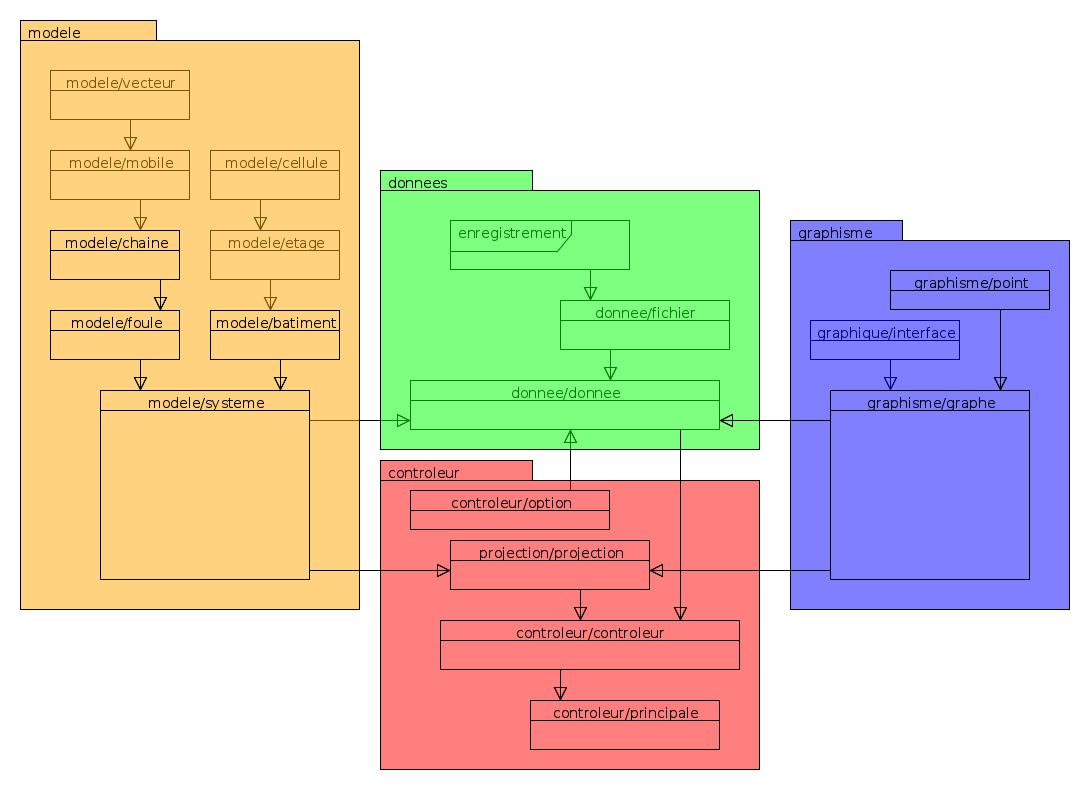
\includegraphics[scale=0.45]{./illustration/classesSimFoule}
\end{center}
%
%
\subsection{diagrammes de séquences}
%e
\newpage
%
\subsubsection{Principale}
%\begin{center}
%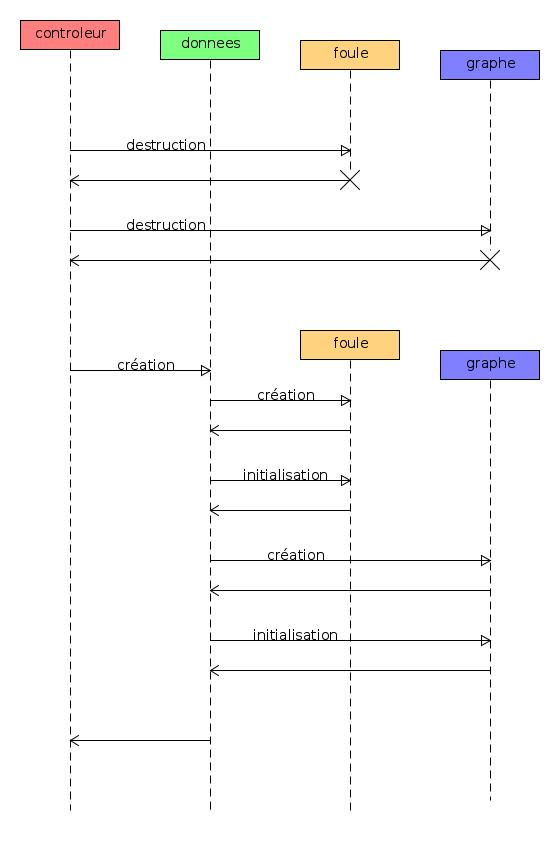
\includegraphics[scale=0.51]{./illustration/sequenceReinitialisation}
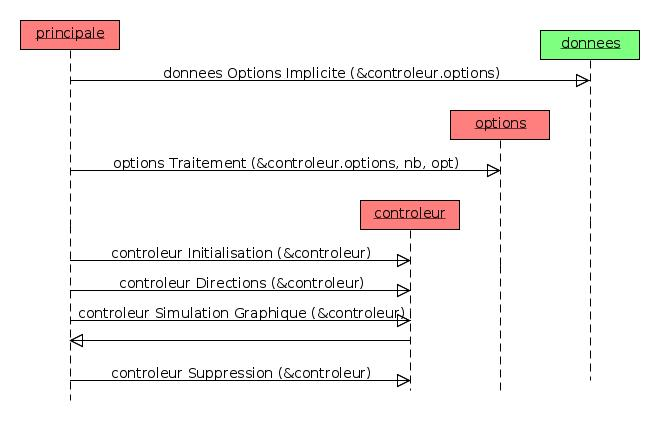
\includegraphics[width=.95\textwidth]{./illustration/sequenceInitialisationPrincipale}

\vspace{.91cm}
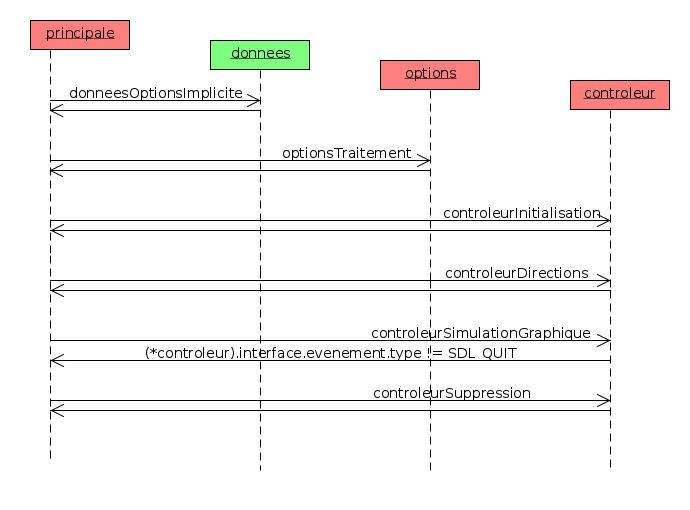
\includegraphics[width=.95\textwidth]{./illustration/sequencePrincipale2}
%\end{center}
%
\subsubsection{Simulation graphique}
%\begin{center}
%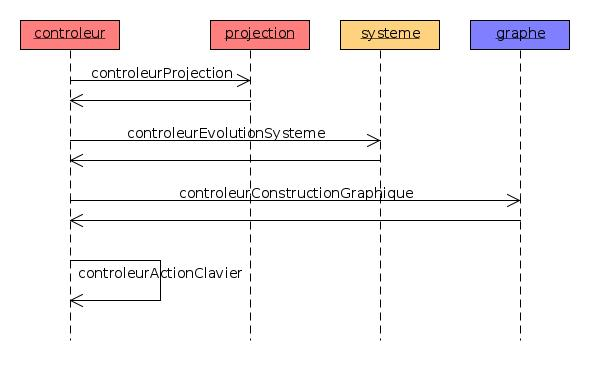
\includegraphics[scale=0.51]{./illustration/sequenceControleur}
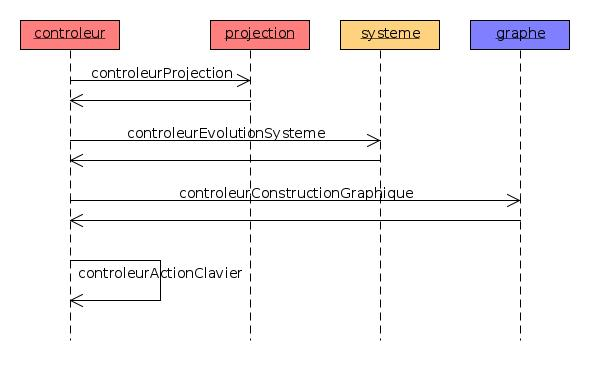
\includegraphics[width=.95\textwidth]{./illustration/sequenceControleur}
%\end{center}
%
\newpage
%
\subsubsection{Réinitialisation}
%\begin{center}
%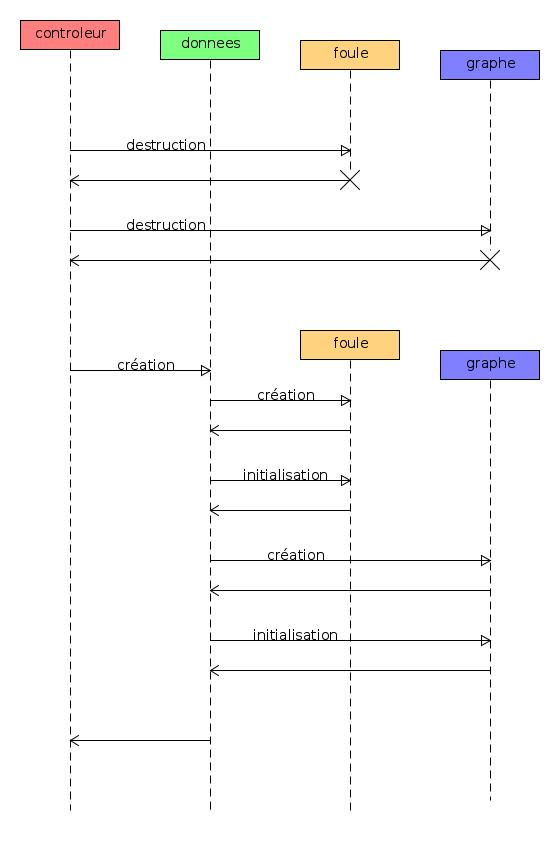
\includegraphics[scale=0.51]{./illustration/sequenceReinitialisation}
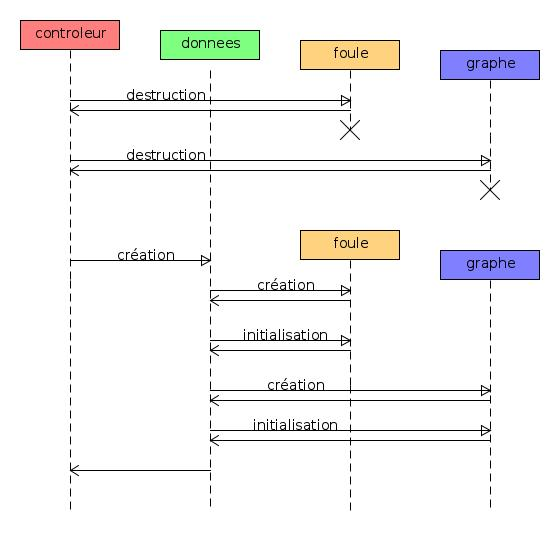
\includegraphics[width=.95\textwidth]{./illustration/sequenceReinitialisation2}
%\end{center}

%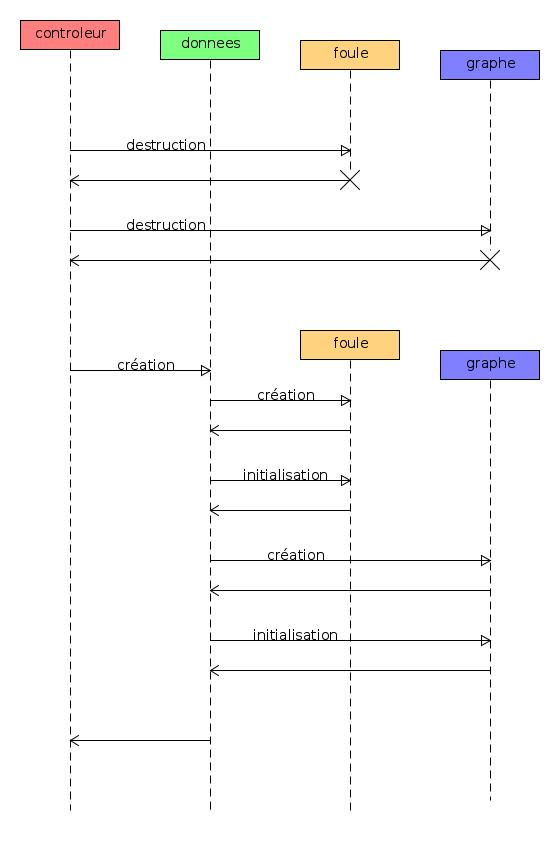
\includegraphics[scale=0.51]{./illustration/sequenceReinitialisation}
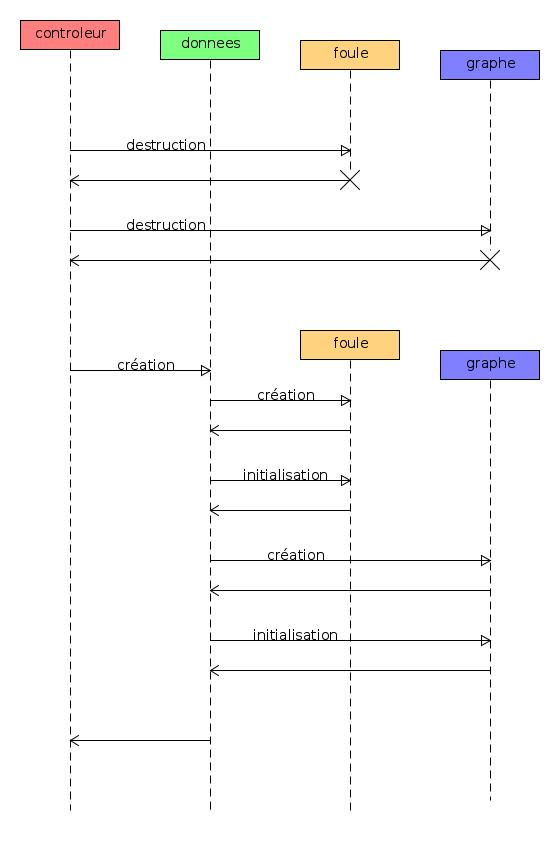
\includegraphics[width=.95\textwidth]{./illustration/sequenceReinitialisation}
%\end{center}
%
%%%%%%%%%%%%%%%%%%%%%%%%%%%%%%%%%%%%%%%%%%%%
%%%%%%%%%%%%%%%%%%%%%%%%%%%%%%%%%%%%%%%%%%%%
%\begin{itemize}[leftmargin=2cm]
%\item \texttt{gras} : texte
%\end{itemize}



%%%%%%%%%%%%%%%%%%%%%%%%%%%%%%%%%%%%%%%%%%%%%%%%%%%%%%%%%%%%%%%%%%%%%%%%%%%%%%%%%%%%%

%
%%%%%%%%%%%%%%%%%%%%%%%%%%%%
\section{Valeurs implicites}
%%%%%%%%%%%%%%%%%%%%%%%%%%%%
%
%
\subsection{Réglage de dt, durée et pause}
Une incrémentation du système correspond à une avancée dans le temps de \texttt{dt}.
Empiriquement, un affichage graphique par 30 ms, est obtenue avec une pause de l'ordre de 25 ms. Si à chaque affichage correspond à une dizaine d'incrémentation de dt, 
\begin{center}
	\begin{tabular}{rcl}
	dt $\times$ duree & = & delay\\
	dt $\times$ 10 & = & 0,03\\
	dt & = & 0,003\\
	\end{tabular}
\end{center}
La valeur de {\texttt duree} peut être changée dynamiquement avec les touches {\texttt F9}, {\texttt F10}, {\texttt F11} et {\texttt F12} afin de faire varier la vitese de la simulation. La valeur de dt peut être réglée avec l'option {\texttt dt} au démarrage du programme, celle de delay par l'option {\texttt pause}.

Dans SimFoule, la valeurs implicites de pause est égale à 25, les valeurs implicites de {\texttt dt} et {\texttt duree} sont réglées dans le fichier {\texttt donnees/donnes.c}. Ces valeurs peuvent être modifiées suivant les objectifs et les capacités de l'ordinateur.
%
%
%
%
%
\subsubsection{Limitation des valeurs des variables}
%
Au delà de certaines valeurs de certain paramètres dynamiques, la simulation s'éloigne du comportement physique.
\begin{itemize}[label=\ding{32}, leftmargin=2cm]
\item Pour des raisons de discrétisation
\item En raisons de possibles erreurs d'algorithme (Le calcul de plus court chemin est réalisé de manière basique et contient un certain nombre d'imperfection...)
\item En raisons de possibles erreurs d'écriture
\end{itemize}
%
Aussi, le fichier {\texttt donnees/constantes.c} contient des valeurs maximale et minimale de certains paramètres. Ces bornes permettent de consolider le comportement du programme.
%
\subsubsection{Paramètres physiques}
%
%
\subsubsection{Paramètres dynamiques}
%
Au delà de certaines valeurs de certain paramètres dynamiques, la simulation s'éloigne d'une évolution physique réaliste.
\begin{itemize}[label=\ding{32}, leftmargin=2cm]
\item Vitesse des mobiles
\item Distance entre les mobiles
\item Énergie des mobiles
\end{itemize}
%

%%%%%%%%%%%%%%%%%%%%%%%%%%%%%%%%%%%%%%%%%%%%%%%%%%%%%%%%%%%%%%%%%

%
%
%====================== INCLUSION DE LA BIBLIOGRAPHIE ======================
%
%récupérer les citation avec "/footnotemark"
%\nocite{*}
%choix du style de la biblio
\bibliographystyle{plain}
%inclusion de la biblio
\cleardoublepage
\addcontentsline{toc}{chapter}{Bibliographie}
\bibliography{bibliographie.bib}
%\newpage
%\input{./glossaire/glossaire.tex}
%\newpage
%\input{./annexes/annexes.tex}
\end{document}
%%%%%%%%%%%%%%%%%%%%%%%%%%%%%%%%%%%%%%%%%%%%%%%%%%%%%%%%%%%%%%%%%%%%%%%%%%%%%%%%%
